%!TEX root = ../../../main.tex
%%---------------------------------------------------------------------------
\section{Human Machine Interface}
\label{sec:rc_hmi}
%%---------------------------------------------------------------------------
A separate Human Machine Interface (HMI) is developed for controlling the robot cell. This allows the user to control relevant parameters from an intuitive GUI. 

The HMI is implemented as a plugin to RobWorkStudio. This allows the HMI to act alongside the visual representation of the work-cell allowing a real-time simulation of the actions.

Figure \ref{fig:rc_hmi} shows the HMI plugin. All system elements are using the log for error and information messages. The user is able to manually control the robot, conveyor and gripper. Some camera settings can be directly controlled from the HMI and the video feed shows a direct view of either the raw or vision applied image. 

	\begin{figure}[H]
		\centering
	    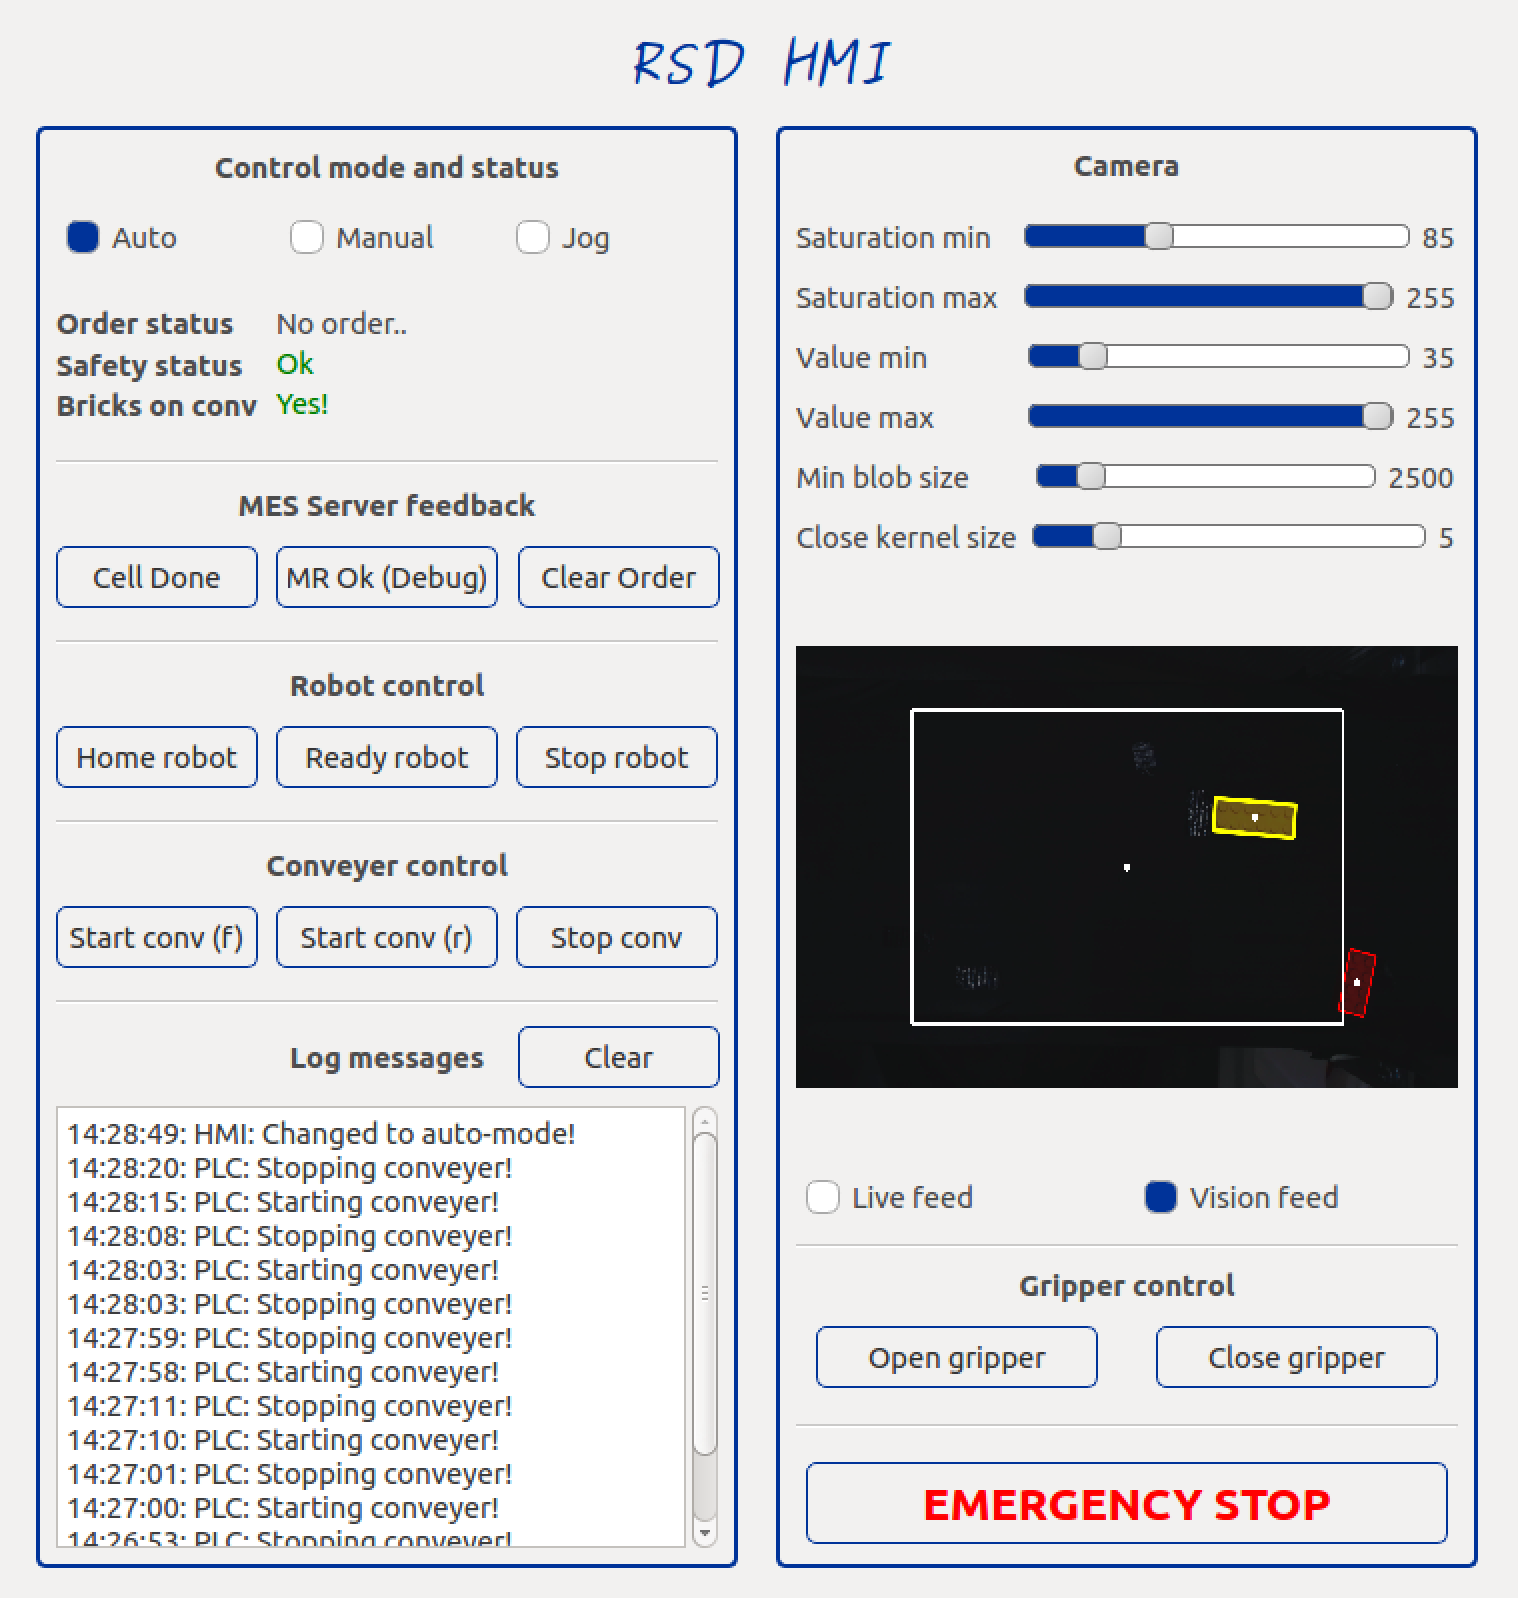
\includegraphics[width=0.9\textwidth]{rc_hmi}
	    \caption{HMI}
		\label{fig:rc_hmi}
	\end{figure}